%
% Also note that the "draftcls" or "draftclsnofoot", not "draft", option
% should be used if it is desired that the figures are to be displayed in
% draft mode.
%\documentclass[draftcls,onecolumn,letterpaper,11pt]{IEEEtran}
%\documentclass[twocolumn,twosides,letterpaper,10pt]{IEEEtran}
\documentclass[conference]{IEEEtran}
%

% common
\usepackage{cite,url,color}
\usepackage{graphicx} %[pdftex]
\graphicspath{{./pdf/}{./jpeg/}{./figs/}{./eps/}}
\DeclareGraphicsExtensions{.pdf,.jpeg,.png,.eps}
% math
\usepackage{multirow}
\usepackage[cmex10]{amsmath}
\usepackage{amssymb,bm}
\interdisplaylinepenalty=2500
% algorithm
%\usepackage{algorithmic}
\usepackage{algpseudocode} % we use this
\newcommand{\algrule}[1][.5pt]{\par\vskip.25\baselineskip\hrule height #1\par\vskip.25\baselineskip}
% subfig
\usepackage[caption=false,font=footnotesize]{subfig}
% theorem
\usepackage[amsmath,thmmarks,hyperref]{ntheorem}
\newtheorem{theorem}{Theorem}
% my command
\newcommand{\ve}[1]{\mathbf{{#1}}}
\newcommand{\abs}[1]{\ensuremath{\vert #1\vert}}
\newcommand{\norm}[1]{\ensuremath{\Vert #1\Vert}}
\newcommand{\diag}{\ensuremath{\mathrm{diag}}}

% correct bad hyphenation here
\hyphenation{op-tical net-works semi-conduc-tor}


\begin{document}

% paper title
\title{Fast Marginalized Block SBL Algorithm}
% author names and IEEE memberships, place (~) in author names to prevent breaking
%\author{Benyuan~Liu$^1$,~Zhilin~Zhang$^2$,~
%        Hongqi~Fan$^1$%
%\thanks{$^1$Benyuan Liu is with The Department of
%Electrical and Communication Engineering, University of Defense Technology,
%Changsha, Hunan, 410074, China. e-mail: liubenyuan@gmail.com}%
%\thanks{$^2$Zhilin Zhang is with The Department of Electrical and Computer
%Engineering, University of California, San Diego, La Jolla, CA 92093-0407,
%USA. e-mail: zhangzlacademy@gmail.com.}%
%\thanks{Manuscript received \today{}.}}
% affiliations
\author{%
\IEEEauthorblockN{Benyuan~Liu,~Hongqi~Fan,~Qiang~Fu}%
\IEEEauthorblockA{%
The Science and Technology on Automatic Target Recognition Laboratory\\
National University of Defense Technology\\
Changsha, Hunan, P. R. China, 410074\\
E-mail: liubenyuan@gmail.com}%
\and
\IEEEauthorblockN{Zhilin~Zhang}%
\IEEEauthorblockA{%
The Emerging Technology Lab\\
Samsung R\&D Institute America - Dallas, 1301 E\\
Lookout Drive, Richardson, TX 75082, USA\\
E-mail: zhilinzhang@ieee.org}%
}

% The paper headers
%\markboth{Submitted to XXXX,~Vol.~X, No.~X, 2013}%
%{Liu \MakeLowercase{\textit{et al.}}: Fast Marginalized Block SBL Algorithm.}

% If you want to put a publisher's ID mark on the page you can do it like
% this:
%\IEEEpubid{0000--0000/00\$00.00~\copyright~2007 IEEE}
% Remember, if you use this you must call \IEEEpubidadjcol in the second
% column for its text to clear the IEEEpubid mark.

% use for special paper notices
%\IEEEspecialpapernotice{(Invited Paper)}

% make the title area
\maketitle

%-------------------------------------------------------------------------
\begin{abstract}
%\boldmath
%% Text of abstract
\end{abstract}

% Note that keywords are not normally used for peerreview papers.
\begin{IEEEkeywords}
\end{IEEEkeywords}



% For peer review papers, you can put extra information on the cover
% page as needed:
\ifCLASSOPTIONpeerreview
\begin{center} \bfseries EDICS Category: SAS-MALN \end{center}
\fi
%
% For peerreview papers, this IEEEtran command inserts a page break and
% creates the second title. It will be ignored for other modes.
\IEEEpeerreviewmaketitle

%-------------------------------------------------------------------------
% main body
The main body of IEEE\cite{Zhang2012a} template.

Compressed sensing\cite{Candes2008a}, as an emerging technology, can recover a signal with less measurements given that the signal is sparse or can be sparse represented in some transformed domain. Compressed sensing based wireless telemonitoring technology\cite{dixon2012compressed,mamaghanian2011compressed,Abdulghani2010,Zhang_TBME2012a,Zhang_TBME2012b} can be viewed as a lossy compression. The block diagram of a typical CS-based wireless telemonitoring is shown in Fig. \ref{fig:diagram}.
\begin{figure}[ht!]
\centering
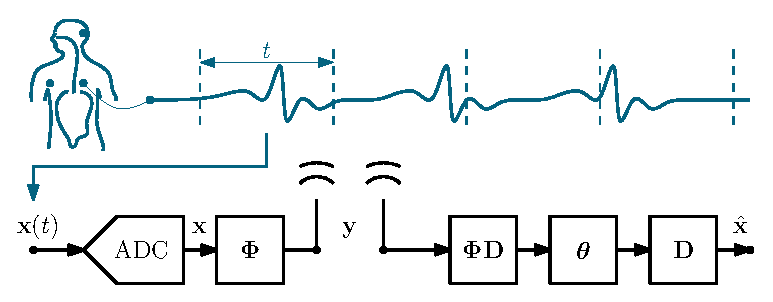
\includegraphics[width=3.4in]{diagram}
\caption{The diagram of a Compressed Sensing (CS) based wireless telemonitoring system. The physiological signal is collected using the sensors attached on the human body. Under the CS paradigm, the signal can be compressed by multiplying an underdetermined matrix. The compressed signal is then transmitted through a wireless network to the data center. The original signal can be reconstructed using a CS recovery algorithm.}%
\label{fig:diagram}
\end{figure}

%\appendices

% use section* for acknowledgment
\section*{Acknowledgement}
The author thanks.

% Can use something like this to put references on a page
% by themselves when using endfloat and the captionsoff option.
\ifCLASSOPTIONcaptionsoff
  \newpage
\fi


% references section
\bibliographystyle{IEEEtran}
\bibliography{bsbl}
%
% <OR> manually copy in the resultant .bbl file
%\begin{thebibliography}{1}

%\bibitem{IEEEhowto:kopka}
%H.~Kopka and P.~W. Daly, \emph{A Guide to \LaTeX}, 3rd~ed.\hskip 1em plus
%  0.5em minus 0.4em\relax Harlow, England: Addison-Wesley, 1999.

%\end{thebibliography}

%===============================================================================
% biography section
%
% If you have an EPS/PDF photo (graphicx package needed) extra braces are
% needed around the contents of the optional argument to biography to prevent
% the LaTeX parser from getting confused when it sees the complicated
% \includegraphics command within an optional argument. (You could create
% your own custom macro containing the \includegraphics command to make things
% simpler here.)
%\begin{IEEEbiography}[{\includegraphics[width=1in,height=1.25in,clip,keepaspectratio]{mshell}}]{Michael Shell}

%\end{IEEEbiography}
% or if you just want to reserve a space for a photo:

% insert where needed to balance the two columns on the last page with
% biographies
%\newpage

% You can push biographies down or up by placing
% a \vfill before or after them. The appropriate
% use of \vfill depends on what kind of text is
% on the last page and whether or not the columns
% are being equalized.

%\vfill

% Can be used to pull up biographies so that the bottom of the last one
% is flush with the other column.
%\enlargethispage{-5in}

% that's all folks
\end{document}


